% Plot Vector Field in LaTeX using Tikz and Pgfplots
% http://latexdraw.com
% 19/10/2019, 19:35

\documentclass{standalone}

\usepackage{tikz}
\usepackage{pgfplots}
\pgfplotsset{compat = newest}
\usepgfplotslibrary{colormaps}

\def\modulus{sqrt(x^2+y^2)}

\begin{document}
    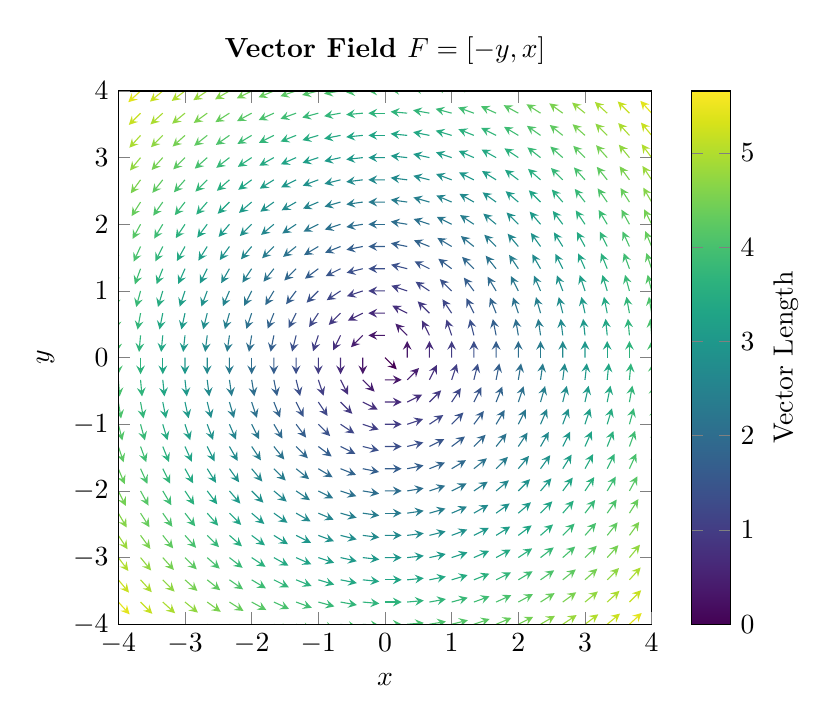
\begin{tikzpicture}
        \begin{axis}[
            xmin = -4, xmax = 4,
            ymin = -4, ymax = 4,
            zmin = 0, zmax = 1,
            axis equal image,
            xtick distance = 1,
            ytick distance = 1,
            view = {0}{90},
            scale = 1.25,
            title = {\bf Vector Field $F = [-y,x]$},
            height=7cm,
            xlabel = {$x$},
            ylabel = {$y$},
            colormap/viridis,
            colorbar,
            colorbar style = {
                ylabel = {Vector Length}
            }
        ]
            \addplot3[
                point meta = {sqrt(x^2+y^2)},
                quiver = {
                    u = {-y/sqrt(x^2+y^2)},
                    v = {x/sqrt(x^2+y^2)},
                    scale arrows = 0.25,
                },
                quiver/colored = {mapped color},
                -stealth,
                domain = -4:4,
                domain y = -4:4,
            ] {0};
        \end{axis}
    \end{tikzpicture}
\end{document}